In a TheHive case, observables can be declared.
Open the Observables list (Case > Observables) to create an observable. You must have permission to administer cases.

The Add observable icon is located on the Observables tab:

\begin{figure}[h]
    \centering
    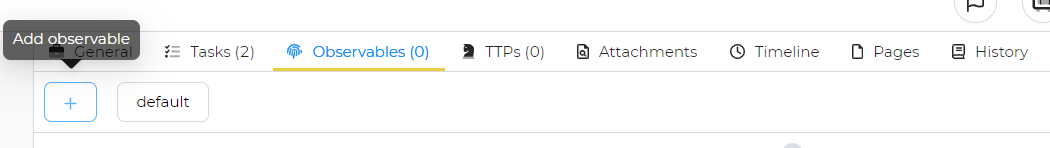
\includegraphics[width=\textwidth]{images/docs/analyst/observable/create-observable-button.png}
    \caption{The structure of the source code of TheHive}
    \label{fig:create-observable-button}
\end{figure}

In the pop-up, you are invited to fill the observable(s) details:
\begin{markdown}
- Type *: The `observable` `dataType` (e.g.: ip, hash, domain, ...)
- Value *: Your observable value (e.g.: 8.8.8.8)
    - One observable per line: Create one observable per line inserted in value field.
    - One single multiline observable: Create one observable, no matter the number of lines (useful for long URLs for example).
- TLP *: Define here the way the information should be shared.
- Is IOC: Check it if this observable is considered as Indicator of Compromission.
- Has been sighted: Has this observable been sighted on your information system.
- Ignore for similarity: Do not correlate this observable with other similar observables.
- Tags **: Tag your observable with insightful information.
- Description **: Description of the observable.
\end{markdown}

\begin{figure}[h!]
    \centering
    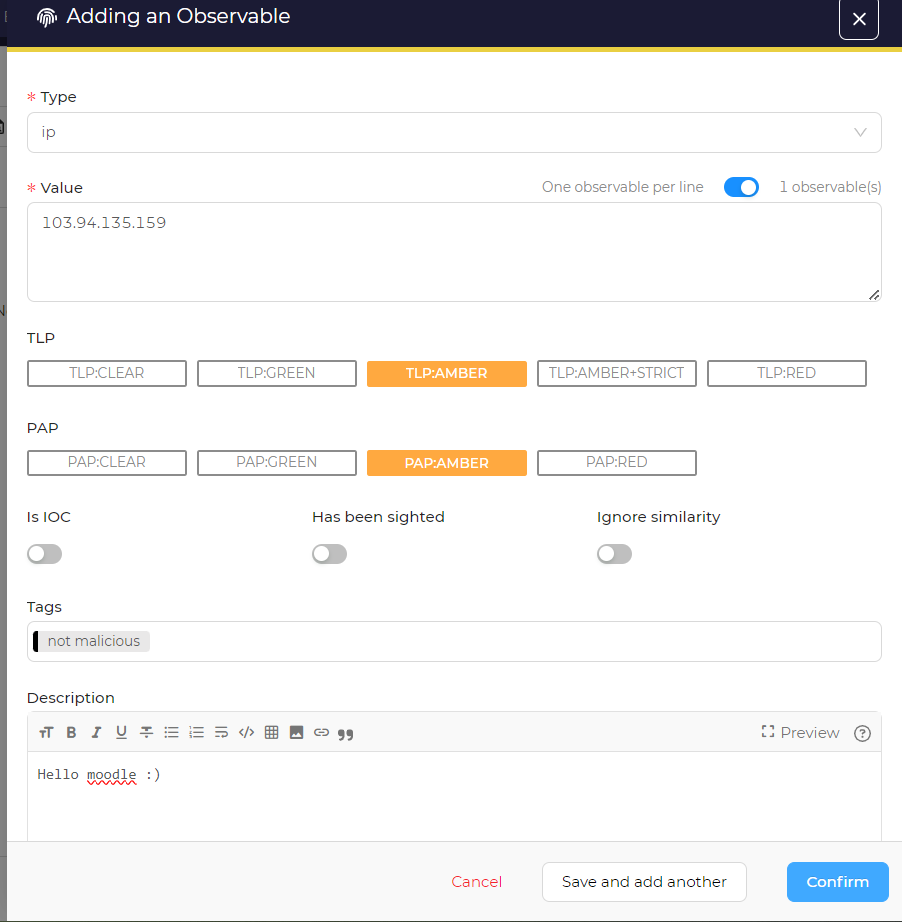
\includegraphics[width=\textwidth]{images/docs/analyst/observable/create-observable.png}
    \caption{The structure of the source code of TheHive}
    \label{fig:create-observable}
\end{figure}

Finally, click on Create Observable(s)